\documentclass[a4paper,11pt]{report}
\usepackage{chuan_math_gkt}
\usetikzlibrary{angles,quotes,intersections,patterns,decorations.pathreplacing}
\chuanexamsetup

\begin{document}
\examfontsize

\examsecret{绝密$\bigstar$启用前}

\examtitle{2025年全国统一高考数学试卷（新高考II卷）}{数\quad 学}

\noticetitle
\begin{examnotice}
\item 答卷前，考生务必将自己的姓名、准考证号填写在答题卡上. 
\item 回答选择题时，选出每小题的答案后，用铅笔把答题卡上对应题目的答案标号涂黑. 如需改动，用橡皮擦干净后，再选涂其他答案标号. 回答非选择题时，将答案写在答题卡上. 写在本试卷上无效. 
\item 考试结束后，将本试卷和答题卡一并交回. 
\end{examnotice}

\examsection{一、单选题：本题共8小题，每小题5分，共40分. 在每小题给出的选项中，只有一项是符合题目要求的. }
\begin{examquestions}
\item 样本数据2，8，14，16，20的平均数为
\fourchoices{$8$}{$9$}{$12$}{$18$}
\item 已知 $z=1+\mathrm{i}$，则 $\dfrac1{z-1}=$
\fourchoices{$-\mathrm{i}$}{$\mathrm{i}$}{$-1$}{$1$}
\item 已知集合 $A=\{-4,0,1,2,8\}$，$B=\{x\mid x^3=x\}$，则 $A\cap B=$
\twochoices{$\{0,1,2\}$}{$\{1,2,8\}$}{$\{2,8\}$}{$\{0,1\}$}
\item 不等式 $\dfrac{x-4}{x-1}\geq2$ 的解集是
\twochoices{$\{x\mid -2\leq x\leq1\}$}{$\{x\mid x\leq-2\}$}{$\{x\mid -2\leq x<1\}$}{$\{x\mid x>1\}$}
\item 在 $\triangle ABC$ 中，$BC=2$，$AC=1+\sqrt3$，$AB=\sqrt6$，则 $A=$
\fourchoices{$45^\circ$}{$60^\circ$}{$120^\circ$}{$135^\circ$}
\item 设抛物线 $C:y^2=2px(p>0)$ 的焦点为 $F$，点 $A$ 在 $C$ 上，过 $A$ 作 $C$ 的准线的垂线，垂足为 $B$，若直线 $BF$ 的方程为 $y=-2x+2$，则 $|AF|=$
\fourchoices{$3$}{$4$}{$5$}{$6$}
\item 记 $S_n$ 为等差数列 $\{a_n\}$ 的前 $n$ 项和，若 $S_3=6,S_5=-5$，则 $S_6=$
\fourchoices{$-20$}{$-15$}{$-10$}{$-5$}
\item 已知 $0<\alpha<\pi$，$\cos\dfrac\alpha2=\dfrac{\sqrt5}{5}$，则 $\sin\left(\alpha-\dfrac\pi4\right)=$
\fourchoices{\tallchoice{$\dfrac{\sqrt2}{10}$}}{\tallchoice{$\dfrac{\sqrt2}{5}$}}{\tallchoice{$\dfrac{3\sqrt2}{10}$}}{\tallchoice{$\dfrac{7\sqrt2}{10}$}}
\end{examquestions}
\examsection{二、多选题：本题共3小题，共18分. 在每小题给出的选项中，有多项符合题目要求. }
\begin{examquestions}[start=9]
\item 记 $S_n$ 为等比数列 $\{a_n\}$ 的前 $n$ 项和，$q$ 为 $\{a_n\}$ 的公比，$q>0$. 若 $S_3=7,a_3=1$，则
\twochoices{$q=\dfrac12$}{$a_5=\dfrac19$}{$S_5=8$}{$a_n+S_n=8$}
\item 已知 $f(x)$ 是定义在 $\mathbb R$ 上的奇函数，且当 $x>0$ 时，$f(x)=(x^2-3)e^x+2$，则
\twochoices{$f(0)=0$}{当 $x<0$ 时，$f(x)=-(x^2-3)e^{-x}-2$}{$f(x)\geq2$ 当且仅当 $x\geq\sqrt3$}{$x=-1$ 是 $f(x)$ 的极大值点}
\item 双曲线 $C:\dfrac{x^2}{a^2}-\dfrac{y^2}{b^2}=1(a>0,b>0)$ 的左、右焦点分别是 $F_1,F_2$，左、右顶点分别为 $A_1,A_2$，以 $F_1F_2$ 为直径的圆与 $C$ 的一条渐近线交于 $M,N$ 两点，且 $\angle NA_1M=\dfrac{5\pi}{6}$，则
\onechoices{$\angle A_1MA_2=\dfrac\pi6$}{$|MA_1|=2|MA_2|$}{$C$ 的离心率为 $\sqrt{13}$}{当 $a=\sqrt2$ 时，四边形 $NA_1MA_2$ 的面积为 $8\sqrt3$}
\end{examquestions}
\examsection{三、填空题：本题共3小题，每小题5分，共15分. }
\begin{examquestions}[start=12]
\item 已知平面向量 $\vec a=(x,1),\vec b=(x-1,2x)$，若 $\vec a\perp(\vec a-\vec b)$，则 $|\vec a|=\blank$. 
\item 若 $x=2$ 是函数 $f(x)=(x-1)(x-2)(x-a)$ 的极值点，则 $f(0)=\blank$. 
\item 一个底面半径为 $4\text{ cm}$，高为 $9\text{ cm}$ 的封闭圆柱形容器（容器壁厚度忽略不计）内有两个半径相等的铁球，则铁球半径的最大值为\blank $\text{cm}$. 
\end{examquestions}
\examsection{四、解答题：本题共5小题，共77分. 解答应写出文字说明，证明过程或演算步骤. }
\begin{examanswers}[start=15]
\item（13分）

已知函数 $f(x)=\cos(2x+\varphi)(0\leq\varphi<\pi)$，$f(0)=\dfrac12$. 

（1）求 $\varphi$；

（2）设函数 $g(x)=f(x)+f\left(x-\dfrac\pi6\right)$，求 $g(x)$ 的值域和单调区间. 
\item（15分）

已知椭圆 $C:\dfrac{x^2}{a^2}+\dfrac{y^2}{b^2}=1(a>b>0)$ 的离心率为 $\dfrac{\sqrt2}{2}$，长轴长为4. 

（1）求 $C$ 的方程；

（2）过点 $(0,-2)$ 的直线 $l$ 与 $C$ 交于 $A,B$ 两点，$O$ 为坐标原点，若 $\triangle OAB$ 的面积为 $\sqrt2$，求 $|AB|$. 
\item（15分）

如图，在四边形 $ABCD$ 中，$AB\parallel CD$，$\angle DAB=90^\circ$，$F$ 为 $CD$ 的中点，点 $E$ 在 $AB$ 上，$EF\parallel AD$，$AB=3AD,CD=2AD$，将四边形 $EFDA$ 沿 $EF$ 翻折至四边形 $EFD'A'$，使得面 $EFD'A'$ 与面 $EFCB$ 所成的二面角为 $60^\circ$. 

\noindent\begin{minipage}[t]{0.64\linewidth}
（1）证明：$A'B\parallel$ 平面 $CD'F$；

（2）求面 $BCD'$ 与面 $EFD'A'$ 所成的二面角的正弦值. 
\end{minipage}\hfill
\begin{minipage}[t]{0.30\linewidth}
\vspace{-2em}
\centering
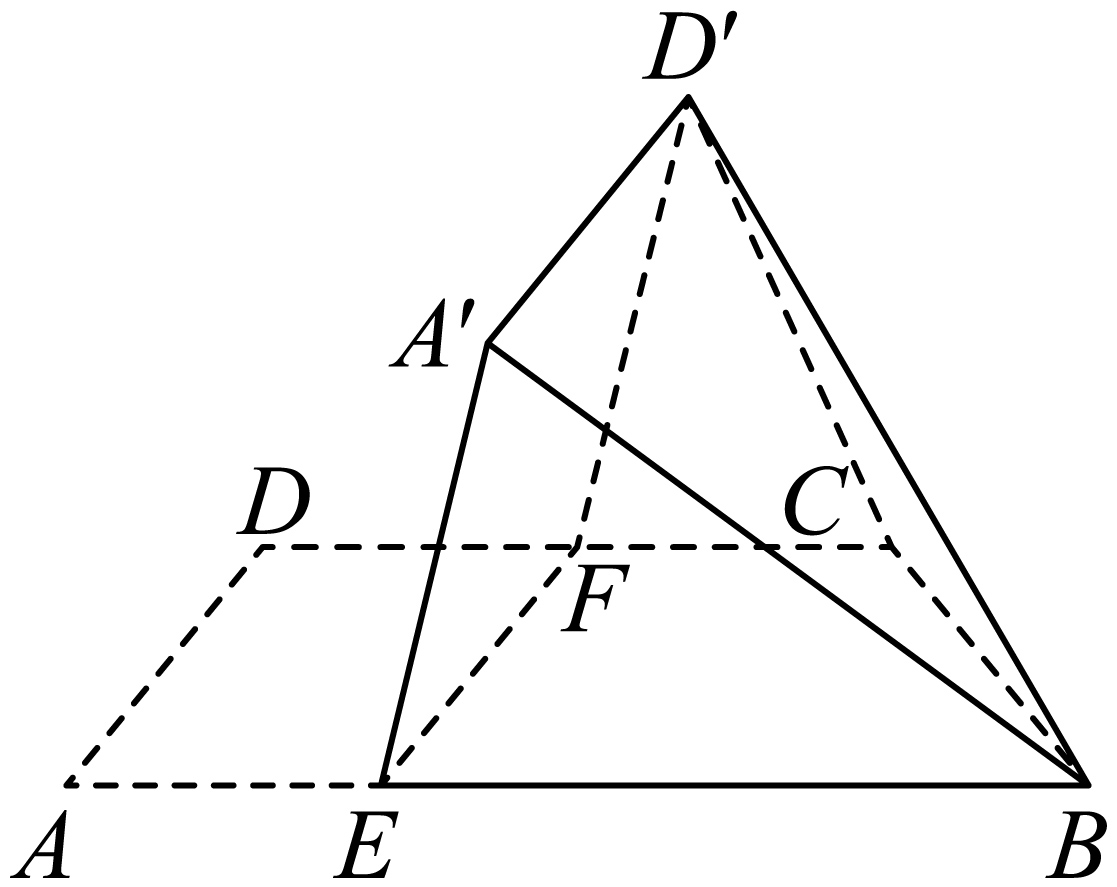
\includegraphics[width=\linewidth]{figures/2025_xgk2_q17.png}
\end{minipage}
\item（17分）

已知函数 $f(x)=\ln(1+x)-x+\dfrac12x^2-kx^3$，其中 $0<k<\dfrac13$. 

（1）证明：$f(x)$ 在区间 $(0,+\infty)$ 存在唯一的极值点和唯一的零点；

（2）设 $x_1,x_2$ 分别为 $f(x)$ 在区间 $(0,+\infty)$ 的极值点和零点. 

（i）设函数 $g(t)=f(x_1+t)-f(x_1-t)$，证明：$g(t)$ 在区间 $(0,x_1)$ 单调递减；

（ii）比较 $2x_1$ 与 $x_2$ 的大小，并证明你的结论. 
\item（17分）

甲、乙两人进行乒乓球练习，每个球胜者得1分，负者得0分. 设每个球甲胜的概率为 $p\left(\dfrac12<p<1\right)$，乙胜的概率为 $q$，$p+q=1$，且各球的胜负相互独立. 对正整数 $k\geq2$，记 $p_k$ 为打完 $k$ 个球后甲比乙至少多得2分的概率，$q_k$ 为打完 $k$ 个球后乙比甲至少多得2分的概率. 

（1）求 $p_3,p_4$（用 $p$ 表示）；

（2）若 $\dfrac{p_4-p_3}{q_4-q_3}=4$，求 $p$；

（3）证明：对任意正整数 $m$，$p_{2m+1}-q_{2m+1}<p_{2m}-q_{2m}<p_{2m+2}-q_{2m+2}$. 
\end{examanswers}

\end{document}
